\chapter{Attenuation Constant in Waveguides}
In this chapter, we will discuss the attenuation constant which was studied in the last chapter. In practice, the material with which the waveguide is made is not an ideal conductor. So, we have ohmic losses in the walls of the waveguide and also the dielectric which is filling the waveguide may not be ideal, and because of that, we may have dielectric losses in the dielectric.

Last time, we saw that the attenuation constant due to two components \textbf{(i) the finite conductivity of the walls and (ii) the finite conductivity of the dielectric filling the waveguide}, which were treated independently. So we calculate the attenuation constants due to each of these components and then we determine the total attenuation constant as the sum of the two attenuation constants under the assumption that the losses are very small in a good waveguide.

Again, in the previous chapters, we calculated the attenuation constant due to dielectric material, thereby introducing the concept of \emph{complex permittivity}\index{complex permittivity}. Therefore, if we replace the dielectric constant with the complex dielectric constant for the medium in the dispersion relation, and then separate the real and imaginary parts, we can get the attenuation constants due to the dielectric losses.

We can then develop a framework for calculating the dielectric constant due to the finite conductivity of the walls and the waveguide.

Hence in this chapter, we will look at two cases which are:
\begin{enumerate}[(i)]
\item the \emph{parallel plane waveguide}\index{parallel plane waveguide} in \textbf{TEM mode}\index{tem mode} and
\item the \emph{rectangular waveguide}\index{rectangular waveguide} in $\boldsymbol{TE_{10}}$ \textbf{mode}
\end{enumerate}

\section{Attenuation Constant For TEM Mode in Parallel Plane Waveguide}
\begin{figure}[h]
\centering
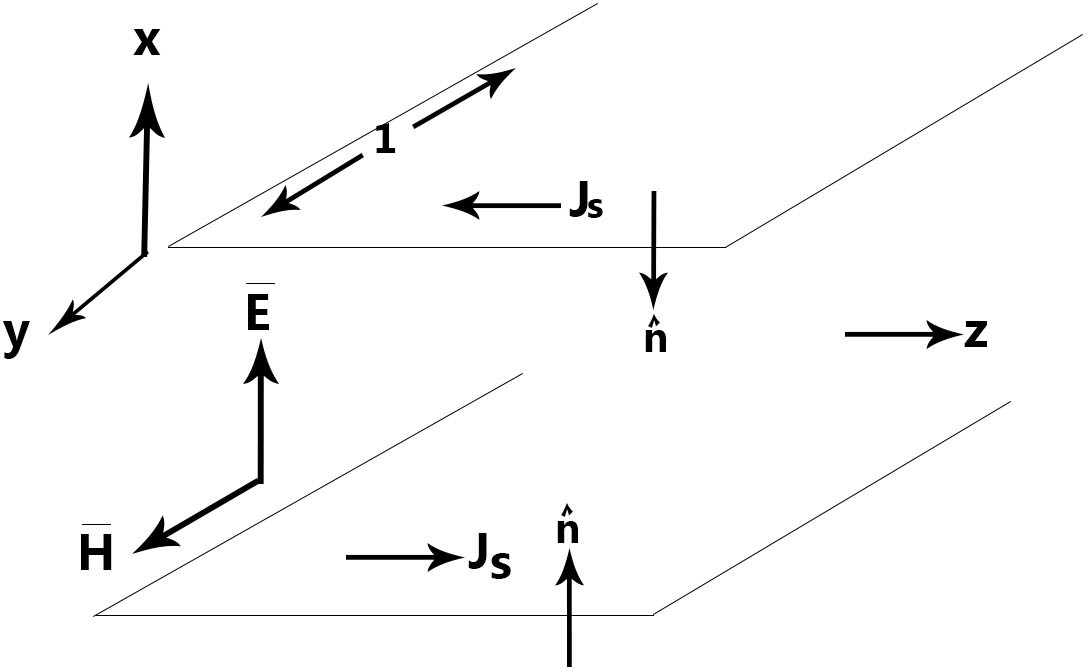
\includegraphics[width=0.8\linewidth]{./graphics/411}
\caption{Propagation of fields inside a parallel plane waveguide operating in TEM mode}
\label{fig:elcture2imageb}
\end{figure}

For the calculation of attenuation constant $\alpha_c$  for TEM in a parallel waveguide to be done, solving for $\alpha_c$ brings to light when we use structures like coaxial cables\index{coaxial cable} and parallel wire transmission lines, and how the losses are calculated. We have seen the calculation of the losses from the knowledge of resistance and conductance in transmission lines. However, we ask a question \emph{how do we know the resistance and conductance in this line?} Essentially starting from the fields, we can calculate how the losses occur in these conducting surfaces.

Now, let us consider a parallel plane waveguide\index{parallel plane waveguide} with a wave propagating in the z-direction as shown in figure~\ref{fig:elcture2imageb} in the TEM mode. For this case, we say $\bar{E}$ is in the x direction and $\bar{H}$ is in the y direction of the coordinate axis. For this mode, the ratio of the $\bar{E}$ and $\bar{H}$ fields is equal to the intrinsic impedance\index{intrinsic impedance} of the medium filling the waveguide so we have a relation between $\bar{E}$ and $\bar{H}$ as:
\begin{dmath*}
\text{Intrinsic impedance}, \eta = \frac{\bar{E}}{\bar{H}}
\end{dmath*}

If we express the electric field $\bar{E}$ as some amplitude $E_0$, then the electric and magnetic fields are given as:
\begin{align*}
\bar{E} &= E_0 e^{-j\beta }\hat{x}\\
\bar{H} &= \frac{E_0}{\eta} e^{-j\beta z}\hat{y}
\end{align*}
Again, the waveguide is infinite in the y direction, so the attention given by the relation, is used to find the total power carried by the waveguide.
\begin{align}
\alpha = \frac{\text{power decrease per unit length}}{2 \times \text{total power carried by the waveguide}}
\label{eqn:alphac}
\end{align}

The power will be infinite since the cross-section of the waveguide is infinite i.e. y tends to $\infty$. The losses will be infinite and we will not get a definite or meaningful answer. So we define an attenuation, $\alpha_{c}$ by the unit width of this waveguide. We take a piece of the waveguide that is of unit length in the y direction i.e. (1) in the y direction. Now begs the question, \emph{what is the power loss in the unit length of the waveguide? What is the power carried by the unit width of the waveguide?} If found we can then calculate the attenuation constant $\alpha_{c}$ of the waveguide.

Now we have $\bar{H}$ which is not varying as a function of y, it is constant for y, with amplitude $\frac{E_0}{\eta}$. Thus, on the top and bottom walls, the magnetic field will be constant for y in the y direction.

As we saw last time, the normal to the surface bounding the electromagnetic wave is as shown in figure~\ref{fig:elcture2imageb}. Thus, we can express the surface current in terms of the normal as $\hat{n}\times\bar{H}=\bar{J_s}$ and determine the direction of $\bar{J_s}$ (shown by the arrows in figure~\ref{fig:elcture2imageb}). This shows that the amplitude of $\bar{J_s}$ is exactly the same amplitude with $\frac{E_0}{\eta}(\bar{H})$. For the TEM mode in the parallel plane waveguide, the fields and currents inside the waveguide can be visualized as shown in figure~\ref{fig:elcture2imageb} and these fields propagate with the phase velocity inside the waveguide in the z-direction.

Also, all the fields, $\bar{E}$ and $\bar{H}$ are going to have a sinusoidal variation as a function of time. If we consider any location on the conducting plane, the fields, $\bar{E}$ and $\bar{H}$ as well as the current $\bar{J_s}$ would vary sinusoidally as a function of time. So, if we take the peak amplitude, $E_0$ and $\frac{E_0}{\eta}$ of $\bar{E}$ and $\bar{H}$ and find out the root-mean-square (RMS) value of the fields and the RMS value of the surface currents, we can get the average power lost and average power carried by the waveguide. So for the unit width of the waveguide, the power carried by the waveguide per unit width is $\frac{\mathfrak{Re}\lbrace E \times H^*\rbrace}{2}$ integrated over the cross-section of height (a or d) and width of the waveguide (unit width). So, let us say the height of the waveguide is given as a, then the power carried by the waveguide per unit width.

\begin{equation}
W=\int_{x=0}^{a}\int_{y=0}^{1} \frac{1}{2}\mathfrak{Re}\lbrace\bar{E} \times \bar{H}^\ast\rbrace dxdy
\label{eqn:powerparawaveguide}	
\end{equation}
For the TEM mode, $\bar{E}$ is in the x direction and $\bar{H}$ is in the y direction, so the power flow is in the z-direction.

From equation~\eqref{eqn:powerparawaveguide}, $\bar{E} \times \bar{H}^\ast = \bar{E} \times \frac{\bar{E}^\ast}{\eta}$. If we consider the dielectric filling the waveguide as an ideal dielectric, $\eta$ is a real quantity, then the power carried by the waveguide per unit width is given as:
\begin{dmath}
W = \int_{x=0}^{a}\int_{y=0}^{1}\frac{1}{2}\mathfrak{Re}\left\lbrace E_0 \frac{E_0^\ast}{\eta}\right\rbrace dxdy
= \frac{\left|E_{0}\right|^2}{2\eta}\int_{x=0}^{a}\int_{y=0}^{1}dxdy 
= \frac{|E_0|^2a}{2\eta}
\label{eqn:powercarriedperunitwidth}
\end{dmath}

This is the total power carried by the TEM mode per unit width of the waveguide. The second quantity we need to determine is the power loss per unit length of the waveguide. As we have seen earlier, to determine the power loss, we need to visit the concept of \emph{surface resistance}\index{surface resistance}. If we know the conductivity of the boundary, we can calculate the surface resistance and from the surface resistance, we can calculate the power loss per unit area as:
\begin{equation}
\text{Power loss per unit area} = \frac{1}{2}R_s|\bar{J_s}|^2 
\end{equation}

So power loss per unit length, $-(\derivative{W}{z})$ is determined as the integration over the area made by a length of 1 unit in the z direction and breadth of 1 unit in the y direction (unit area). The magnitude of $ \bar{J_s} $ is the same as that of the magnetic field, so its magnitude will be $ \frac{E_0}{\eta} $ and $H^\ast$ will have a sinusoidal variation in time. So for the per unit length, if we calculate power loss per unit area and integrate it over the unit area would give the total loss per wall. Since there are 2 walls, the total loss will be doubled, that is, for each wall, we calculate power loss per unit length
\begin{equation*}
-\derivative{W}{z} = 2\footnotemark \int_{y=o}^{1} \int_{z=0}^{1}\frac{1}{2}R_s|\bar{J_s}|^2dydz
\end{equation*}
\footnotetext{
This represents the doubling of the power loss per unit length due to the presence of two walls.
}
If we recall, the surface resistance, $R_s$ was the real part of the intrinsic impedance of the conducting wall. Again, the intrinsic impedance of the conducting wall is given as
\begin{dmath*}
\eta_c = \sqrt{\frac{j\omega\mu}{\sigma}}
= \sqrt{\frac{\omega\mu}{2\sigma}}+j\sqrt{\frac{\omega\mu}{2\sigma}}\quad\text{where }\sqrt{\frac{\omega\mu}{2\sigma}}\text{ = }R_s\text{ and }j\sqrt{\frac{\omega\mu}{2\sigma}}\text{ = }jX_s
= R_s + jX_s
\end{dmath*}
Where $R_s$ is the surface resistance\index{surface resistance} and $X_s$ is the surface reactance. Back to the power loss per unit width, if we substitute for $R_s$ and $|\bar{J_s}|^2$ in the equation, we get
\begin{dmath}
-\derivative{W}{z} = \int_{y=o}^{1} \int_{z=0}^{1}\frac{1}{2}\sqrt{\frac{\omega\mu}{2\sigma}}\times\frac{|E_0|^2}{\eta}dydz
= \sqrt{\frac{\omega\mu}{2\sigma}}\times\frac{|E_0|^2}{\eta}
\label{eqn:powerlossperunitlength}
\end{dmath}
Equation~\eqref{eqn:powerlossperunitlength} is the power loss per unit length of the waveguide. So, we have the quantities which are needed for the calculation of the attenuation constant.

Thus subsituting for values in equation~\eqref{eqn:alphac} the attenuation constant, $\alpha_c$ is given as 
\begin{dmath}
\alpha_c = \frac{\sqrt\dfrac{\omega\mu}{2 \sigma}\times\dfrac{|E_0|^2}{\eta}}{2 \times \dfrac{|E_0|^2 a}{2 \eta}}
= \frac{2}{a}\sqrt{\frac{\omega\mu}{2\sigma}}=\frac{1}{a}\sqrt{\frac{\omega\mu}{2\sigma}}
\end{dmath}

This gives us the attenuation constant of the parallel plane waveguide. $\omega$ is the frequency, $a$ is the height of the waveguide, $\mu$ is the permeability of the dielectric, and $\sigma$ is the conductivity of the parallel planes. There are some observations we can make from this equation. 
\begin{enumerate}[(i)]
\item The attenuation constant is inversely proportional to the height of the waveguide. This makes sense because if we consider the parallel plane waveguide since the magnetic field does not vary as a function of height, no matter the separation of the two planes, the power loss per unit length is the same as it does not change. However, the power carried by the waveguide is affected in that it increases. But the power loss per unit length does not change and it is small. As a result, the attenuation constant reduces with increasing height, $a$.
\item The attenuation constant is inversely proportional to the conductivity, $\sigma$. That, we understand, because if we have a good conductor, as the conductivity becomes large, the attenuation gets smaller since there will be less loss in the limit, that is, as $\sigma$ tends to $\infty$, $\alpha_{c}$ tends to 0. So, a waveguide made of an ideal conductor will have zero attenuation constant.
\item Attenuation constant is directly proportional to frequency, in that, as frequency increases, attenuation constant increases and vice versa. Thus, at high frequencies, the loss becomes excessive and the signal cannot be fed effectively.

This explains why in coaxial cables\index{coaxial cable}, at low frequencies, the attenuation constant is manageable whereas high frequencies create a low-pass filtering effect smoothening signals because of too much losses. Essentially, when the same structure is used to carry the signal at high frequencies, the loss becomes excessive, so the signal cannot be transmitted efficiently from one point to the other. Alternatively, suppose we had to send a broadband signal\footnote{
A broadband signal is one that occupies a very large bandwidth
}\index{broadband signal} using the structure, the lower end of the frequency spectrum will pass through the structure, but the higher end of the spectrum will not pass through the structure rather, its amplitude will be reduced (just like a low pass filter).
\end{enumerate}

With these observations, we conclude on the propagation of broadband signals in a guiding structure, such that invariably there is low pass filtering and a distorted signal i.e. there will be blurring of the sharp edges of the signal in time. Therefore, broadband signals get smoothed out because of low pass filtering action caused by the lossy behaviour of the waveguide which varies with frequency and so an increase in frequency will lead to a high loss for the same waveguide structure.

\section{Attenuation Constant for $TE_{10}$ mode in a Rectangular Waveguide}
For this mode let us make some recapitulations. The $TE_{10}$ mode is the dominant mode in a rectangular waveguide. The fields are given as
\begin{align*}
E_{x} &= E_{z} = H_{y} = 0\\
E_{y} &= \dfrac{-j\omega\mu a }{\pi} C\sin \dfrac{\pi a}{x} e ^{-j\beta z}\\
H_{x} &= \dfrac{-j\omega a}{\pi} C \sin\dfrac{\pi a}{x}
e^{-j\beta z}\\
H_{z} &= C\cos \dfrac{\pi x}{a} e^{-j\beta z}
\end{align*}
In the previous chapters, we saw the current distribution because of these fields. Now we use these fields to calculate the power carried by the waveguide, the loss in the four walls of the waveguide and then we calculate the attenuation constant.

Consider the rectangular waveguide operating in $TE_{10}$ shown in figure~\ref{fig:lectureimage21}. First, we calculate the total power since the area of the cross-section is known.
\begin{figure}[H]
\centering
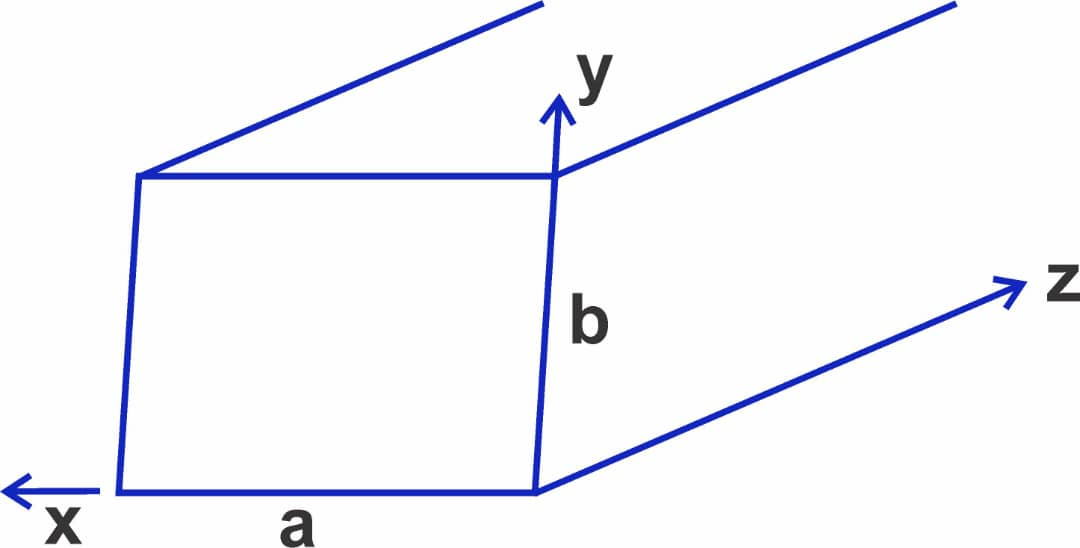
\includegraphics[width=1\linewidth]{./graphics/lecture-image-21.jpg}
\caption{$TE_{10}$ mode propagation in a rectangular waveguide}
\label{fig:lectureimage21}
\end{figure}

We take per unit length of the waveguide in the z-direction. Calculate the loss per unit length, from the same argument, at every location the field is going to sinusoidally as a function of time. We take the peak value of the magnetic field and just take the RMS value from there and then we can calculate the power loss by integrating over the length of the waveguide.

First, we take total power or power carried:
\begin{dmath*}
W= \int_{x=0}^{a}\int_{y=0}^{b}\frac{1}{2}\mathfrak{Re}\lbrace\bar{E} \times H^*\rbrace dxdy
\end{dmath*}
$E = E_y \hat{y}$ and $H = H_x\hat{x} + H_z\hat{z}$, such that $E_y\times H_x^\ast\approx j\times(-j) = -1$ is real while $E_y\times H_z^\ast \approx j \times 1$ is imaginary. So only $E_y\times H_x^*$ gives real power flow. 

Therefore,
\begin{dmath*}
W= \int_{x=0}^{a}\int_{y=0}^{b}\frac{1}{2}\mathfrak{Re}\{E_yH_x^*(-\hat{z})+(E_yH_z^*)\}dxdy
= \int_{x=0}^{a}\int_{y=0}^{b}\frac{1}{2}\frac{\omega\mu a}{\pi}.\frac{\beta a}{\pi}c^2{\sin}^2(\frac{\pi x}{a})dxdy
=\frac{\omega\mu\beta a^2c^2}{2\pi^2}.b\int_{x=0}^{a}{\sin}^2(\frac{\pi x}{a})dx
=\frac{\omega\mu\beta a^3bc^2}{4\pi^2}
\end{dmath*}
By knowing the fields for $TE_{10}$ mode, we can calculate the total power carried by the waveguide. Power calculation for the loss in the waveguide is rather tedious because, in the case of the parallel plane waveguide, we had only two planes and the current distribution was simple and the current was moving only in the z direction, so we could integrate very easily.

In the case of the rectangular waveguide, the current which is flowing on the surface is rather complicated. We showed in the previous chapters that it was some kind of blooming and closing flower on the two alternate walls of the rectangular waveguide. To revisit our discussion in those chapters, consider figure~\ref{fig:lecture2-image-a}.
\begin{figure}[h]
\centering
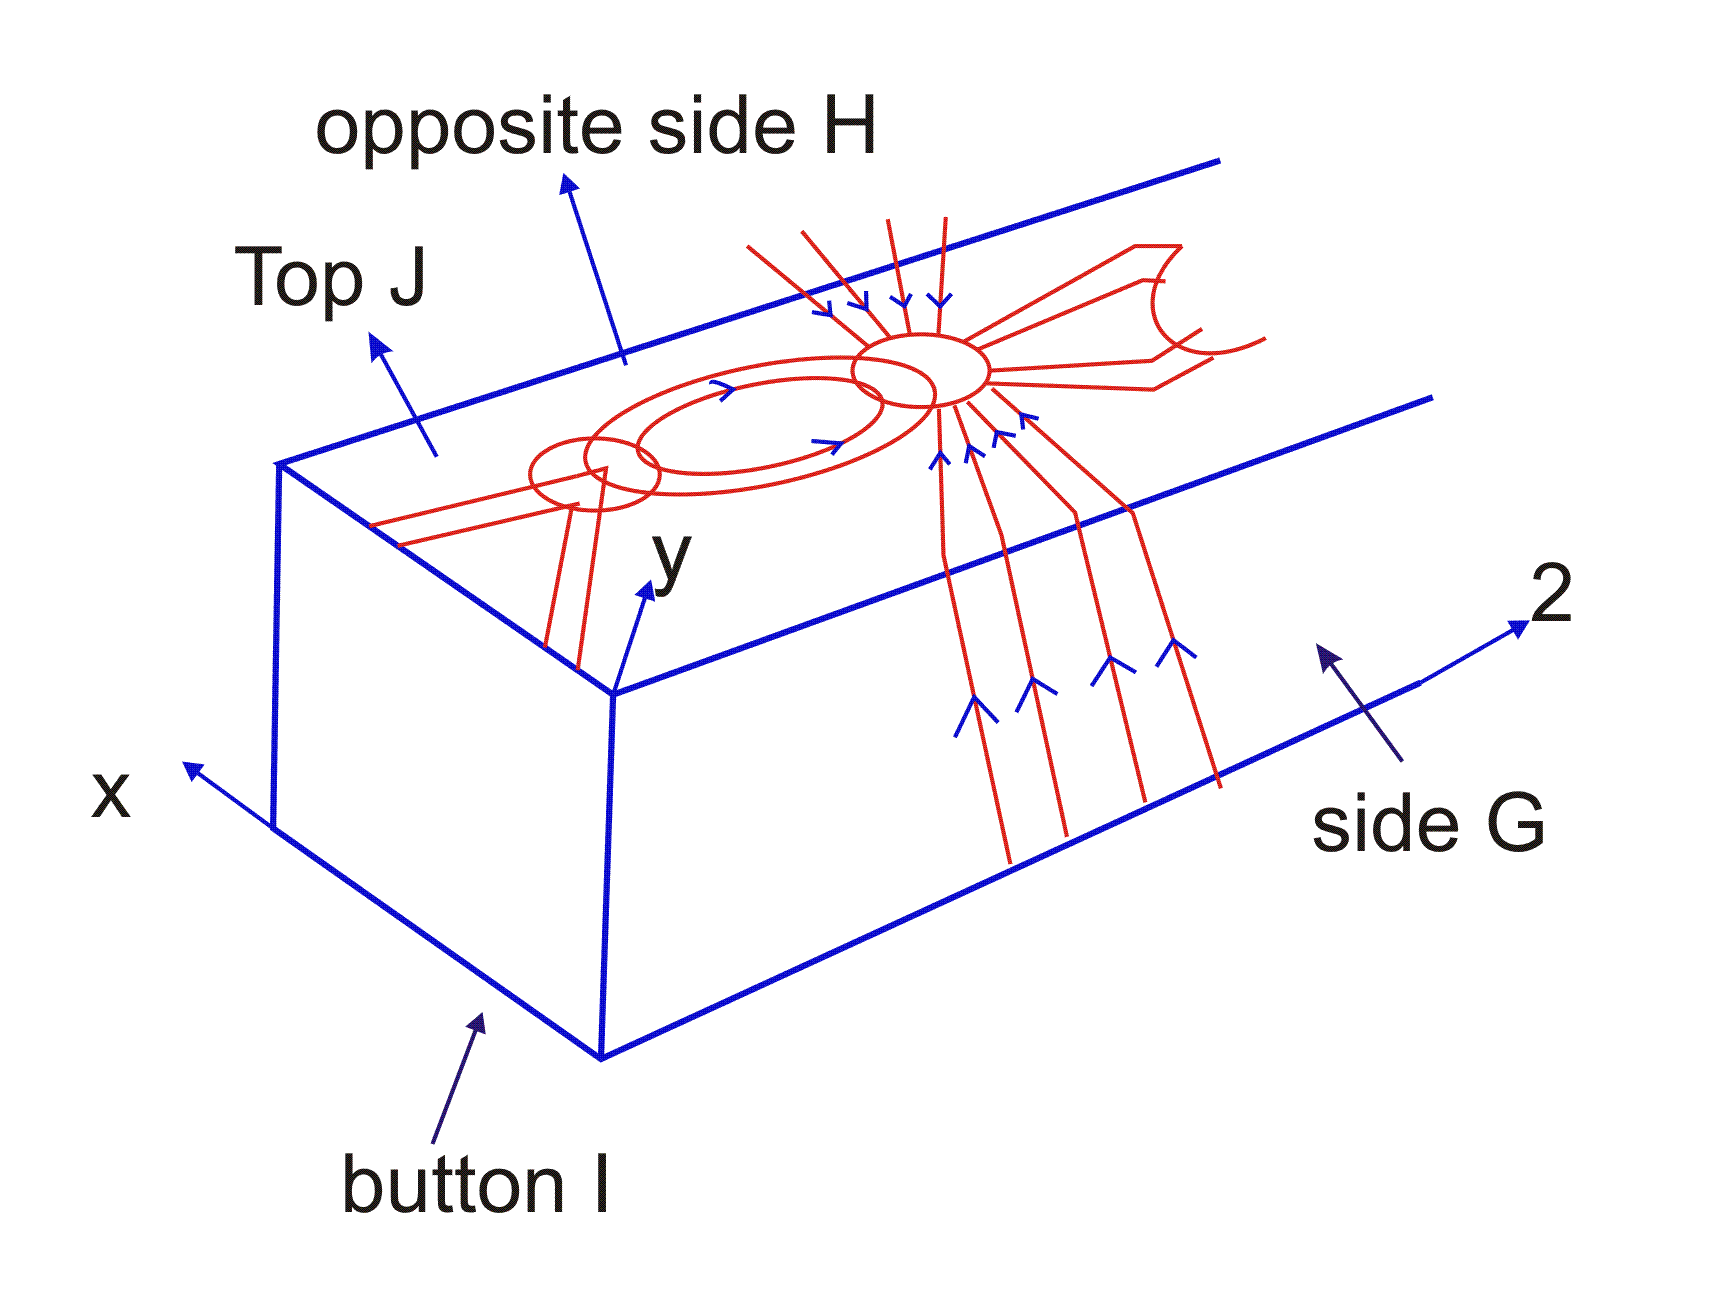
\includegraphics[width=1\linewidth]{./graphics/lecture2-image-a.png}
\caption{The direction of magnetic and electric fields viewed from the surface of a rectangular waveguide}
\label{fig:lecture2-image-a}
\end{figure}

On side walls G and H, the surface current is y-oriented as shown in figure~\ref{fig:lecture2-image-a}. It is contributed by the magnetic field component, $H_z$ since $H_x$ is zero at $x=0$ or $x=a$ (see equation~\eqref{eqn:hxrecte10}). On the top and bottom walls J and I, we have the surface current direction in x and z since both $H_x$ and $H_z$ are non-zero at $y=0$ and $y=b$ (see equations~\eqref{eqn:hxrecte10} and~\eqref{eqn:hzrecte10}). Therefore, on sides G and H, we have currents that are only y oriented given as

From this point onward, it becomes feasible to compute the waveguide's loss. However, at this juncture, we possess the two constituent elements of the current. The first current component is oriented in the z-direction and is present at both the top and bottom walls. The second current component is oriented in the x-direction and is also present at the top and bottom walls. To determine the overall current along these walls, it is necessary to perform a vector summation of the two currents on the top and bottom surfaces of the waveguide. Subsequently, by utilizing this combined current, the total loss of the waveguide can be computed.

First, let us calculate the loss for the sidewalls G and H. For the side wall, $H_z=cos(\frac{\pi x}{a})e^{j\beta z}$ at $x=a$ gives current ($\hat{n} \times \bar{H}$) which does not vary with y and at $x=0$ gives current which again does not vary with y. Also, $e^{j\beta z}$ gives sinusoidal variation but we are interested in the amplitude, hence instead of writing $Ce^{-j\beta z}$ with $x=0$ or $x=a$, we take just the C term. So, we calculate the loss in the two walls per unit length of the waveguide as

The computation of loss in the vertical walls is relatively straightforward since we only have one component of the surface current, which is oriented in the y-direction. However, when examining the top surface, we encounter two magnetic field components, namely $H_x$ and $H_z$, present on both the top and bottom surfaces. Hence, it is necessary to determine the aggregate current on this surface and subsequently evaluate the loss for both the top and bottom surfaces. 

For the horizontal walls, $\bar{J_s}$ is a vector quantity now as there are two components in x and z.

From equations~\eqref{eqn:hxrecte10} and~\eqref{eqn:hzrecte10}, we observe that they are not varying as a function of y, so they are the same at $y=0$ or $y=b$ i.e. at the top and bottom walls which are the two horizontal walls.
Equation~\eqref{eqn:lossrecte10} is the total loss in the four walls in terms of the cut-off frequency. So, to calculate the attenuation constant, we require two essential pieces of information: the total power conveyed by the waveguide and the power loss per unit length of the waveguide which have already been determined. With these two quantities known, the attenuation constant of the waveguide can be derived, yielding valuable insights into its characteristics.
With $R_s=\sqrt\frac{\omega\mu}{2\sigma}$ in $\alpha_{c}$ expression, it implies that the higher the frequency, the higher $\alpha_{c}$ and the more the losses. We also know that $\alpha_{c}$ is related to the ratio $\frac{f_c}{f}$. As f tends to $f_c$ becomes very large and when frequency approaches the cut-off frequency, there is no propagation of the mode i.e. the propagation ceases, the power essentially bounces back and forth between the two surfaces and the power is essentially absorbed in the ohmic losses of these walls and the attenuation constant becomes very large.

So having understood these two cases, one was a simple case of the parallel plane waveguide in TEM mode. the other is the rectangular waveguide in $TE_{10}$ mode which is the dominant mode in a rectangular waveguide. We have explained the philosophy of how the attenuated constant is calculated inside the waveguide, and using this philosophy, the attenuation constant can be calculated for any arbitrary mode inside the waveguide.

In summary, the attenuation constant plays a crucial role in waveguiding structures, regardless of the scale of losses involved. Even in cases where losses are minimal, it is desirable to quantify the extent of these losses, necessitating the determination of the attenuation constant in a parallel plane waveguide. We have observed that the attenuation constant of a waveguide comprises two distinct components:
\begin{enumerate}[(i)]
\item due to dielectric loss because of the finite conductivity of the dielectric filling the waveguide
\item due to losses arising from finite conductivity of the conducting boundary.
\end{enumerate}
Under the assumption of small losses in both the dielectric and conductor, we proceed to calculate the attenuation constant attributed to each type of loss separately. Firstly, for dielectric losses, we employ the concept of complex permittivity, wherein the dielectric constant is replaced with a complex dielectric constant in the dispersion relation. By decomposing the complex dielectric constant into its real and imaginary parts, we obtain the attenuation constant due to dielectric losses.

As for conducting losses, we evaluate the total power flow within the waveguide and determine the losses per unit length along the waveguide's walls. Utilizing this information, we can derive the attenuation constant of the waveguide resulting from conducting losses. With this, our discussion on the propagation of normal waves in waveguides concludes.

Throughout this course, we have observed a gradual transition from a wave existing in an unbounded medium to its confinement within increasingly bound structures. Upon reviewing the progression of plane wave propagation, we initially consider a wave in an unbounded medium. Subsequently, we introduce an interface to confine the wave's propagation within a semi-infinite space. Next, two parallel planes are employed to effectively confine the wave between them, resulting in the formation of a structure known as a parallel plane waveguide. To further constrain the wave, we restrict its propagation in the remaining two directions, ultimately trapping it within a closed pipe, referred to as a rectangular waveguide. It is also possible to enclose the structure by closing off the remaining two sides of the pipe, transforming it into a \emph{resonator}\index{resonator}. However, the discussion of resonators falls outside the scope of this course. The transition from an unbounded medium to a bound medium through wave structures elucidates how electromagnetic waves are guided within specific systems. Consequently, waveguides serve as highly valuable devices for efficiently directing electromagnetic waves from one point to another.
